\documentclass[11pt,a4paper]{article}
% Shared preamble for the NAIL094 reports
% Used by every task via % Shared preamble for the NAIL094 reports
% Used by every task via % Shared preamble for the NAIL094 reports
% Used by every task via \input{../../shared/preamble}

\usepackage[T1]{fontenc}
\usepackage[utf8]{inputenc}
\usepackage{lmodern}
\usepackage[margin=2.5cm]{geometry}

\usepackage{amsmath}
\usepackage{amssymb}
\usepackage{booktabs}
\usepackage{float}
\usepackage{graphicx}
\usepackage{listings}
\usepackage{xcolor}
\usepackage{caption}

\usepackage[hidelinks]{hyperref}

\setlength{\parskip}{0.5em}
\setlength{\parindent}{0pt}

% Title fields, set these in the report before \begin{document}
\makeatletter
\newcommand{\reportcourse}[1]{\def\@reportcourse{#1}}
\newcommand{\reporttask}[1]{\def\@reporttask{#1}}
\newcommand{\reportauthor}[1]{\def\@reportauthor{#1}}

\newcommand{\makereporttitle}{%
  \begin{center}
    {\LARGE\bfseries \@reportcourse \par}
    \vspace{0.8em}
    {\Large \@reporttask \par}
    \vspace{0.6em}
    {\normalsize \@reportauthor \par}
  \end{center}
  \vspace{1em}
  \hrule
  \vspace{1.5em}
}
\makeatother

% Inline code
\newcommand{\code}[1]{\texttt{#1}}

% Code listings
\lstdefinestyle{reportcode}{
  basicstyle=\ttfamily\small,
  keywordstyle=\color{blue!60!black},
  commentstyle=\color{gray},
  stringstyle=\color{green!40!black},
  breaklines=true,
  showstringspaces=false,
  frame=single,
  rulecolor=\color{gray!40},
  numbers=none,
}
\lstset{style=reportcode}


\usepackage[T1]{fontenc}
\usepackage[utf8]{inputenc}
\usepackage{lmodern}
\usepackage[margin=2.5cm]{geometry}

\usepackage{amsmath}
\usepackage{amssymb}
\usepackage{booktabs}
\usepackage{float}
\usepackage{graphicx}
\usepackage{listings}
\usepackage{xcolor}
\usepackage{caption}

\usepackage[hidelinks]{hyperref}

\setlength{\parskip}{0.5em}
\setlength{\parindent}{0pt}

% Title fields, set these in the report before \begin{document}
\makeatletter
\newcommand{\reportcourse}[1]{\def\@reportcourse{#1}}
\newcommand{\reporttask}[1]{\def\@reporttask{#1}}
\newcommand{\reportauthor}[1]{\def\@reportauthor{#1}}

\newcommand{\makereporttitle}{%
  \begin{center}
    {\LARGE\bfseries \@reportcourse \par}
    \vspace{0.8em}
    {\Large \@reporttask \par}
    \vspace{0.6em}
    {\normalsize \@reportauthor \par}
  \end{center}
  \vspace{1em}
  \hrule
  \vspace{1.5em}
}
\makeatother

% Inline code
\newcommand{\code}[1]{\texttt{#1}}

% Code listings
\lstdefinestyle{reportcode}{
  basicstyle=\ttfamily\small,
  keywordstyle=\color{blue!60!black},
  commentstyle=\color{gray},
  stringstyle=\color{green!40!black},
  breaklines=true,
  showstringspaces=false,
  frame=single,
  rulecolor=\color{gray!40},
  numbers=none,
}
\lstset{style=reportcode}


\usepackage[T1]{fontenc}
\usepackage[utf8]{inputenc}
\usepackage{lmodern}
\usepackage[margin=2.5cm]{geometry}

\usepackage{amsmath}
\usepackage{amssymb}
\usepackage{booktabs}
\usepackage{float}
\usepackage{graphicx}
\usepackage{listings}
\usepackage{xcolor}
\usepackage{caption}

\usepackage[hidelinks]{hyperref}

\setlength{\parskip}{0.5em}
\setlength{\parindent}{0pt}

% Title fields, set these in the report before \begin{document}
\makeatletter
\newcommand{\reportcourse}[1]{\def\@reportcourse{#1}}
\newcommand{\reporttask}[1]{\def\@reporttask{#1}}
\newcommand{\reportauthor}[1]{\def\@reportauthor{#1}}

\newcommand{\makereporttitle}{%
  \begin{center}
    {\LARGE\bfseries \@reportcourse \par}
    \vspace{0.8em}
    {\Large \@reporttask \par}
    \vspace{0.6em}
    {\normalsize \@reportauthor \par}
  \end{center}
  \vspace{1em}
  \hrule
  \vspace{1.5em}
}
\makeatother

% Inline code
\newcommand{\code}[1]{\texttt{#1}}

% Code listings
\lstdefinestyle{reportcode}{
  basicstyle=\ttfamily\small,
  keywordstyle=\color{blue!60!black},
  commentstyle=\color{gray},
  stringstyle=\color{green!40!black},
  breaklines=true,
  showstringspaces=false,
  frame=single,
  rulecolor=\color{gray!40},
  numbers=none,
}
\lstset{style=reportcode}


\reportcourse{NAIL094 --- Decision Procedures and SAT/SMT Solvers}
\reporttask{Cryptarithms}
\reportauthor{Zerina Ahmetovic}

\begin{document}
\makereporttitle

\section{Task overview}

A cryptarithm is a number puzzle in which an alphabet is used to encode some
numbers of base $k$. The goal is to form a one-to-one function between the
alphabet and the numbers so that the decoded mathematical formula is
satisfied. The size of the alphabet is bounded by $k$. Numbers cannot have leading zeroes. The classic example is
\[
\begin{array}{r@{\quad}r}
  \texttt{ SEND} & 9567 \\
  \texttt{+MORE} & +1085 \\
  \hline
  \texttt{MONEY} & 10652
\end{array}
\]

The basic constraint has the form $w_1 \square w_2 \square \dots \square w_n = s$,
where the $w_i$ and $s$ are words and $\square$ denotes addition or
subtraction.

The base is a parameter of the program, and the encoding described below is
written for a general $k$. Every other place where a value is needed and none is given, in
the text and in the tables alike, the base is naturally $k = 10$.

Several features are required of the program:

\begin{itemize}
  \item support formulas built from such equations, where \code{||} or
  \code{OR} denotes a disjunction, \code{\&\&} or \code{AND} a conjunction and
  \code{NOT} a negation, or another reasonable format may be chosen;
  \item make the unique interpretation of characters as digits optional, that
  is allow also the case when two characters can represent the same digit;
  \item check if the solution is unique, count or enumerate all solutions, as
  an option;
  \item test the program on instances taken from external
  collections\footnote{\url{https://tamura70.gitlab.io/web-puzzle/cryptarithm/}}
  and on more complex formulas which use these equations.
  \item measure how long it takes to solve
  the following problem, an equation with 41 addends:
  \begin{quote}\small\ttfamily
  SO+MANY+MORE+MEN+SEEM+TO+SAY+THAT+THEY+MAY+SOON+TRY+TO+\\
  STAY+AT+HOME+SO+AS+TO+SEE+OR+HEAR+THE+SAME+ONE+MAN+TRY+\\
  TO+MEET+THE+TEAM+ON+THE+MOON+AS+HE+HAS+AT+THE+OTHER+TEN\\
  =TESTS
  \end{quote}
\end{itemize}



\section{Analysis}

\subsection*{Variables}

Every letter is represented by $k$ Boolean variables, one for each digit, of
which one is true. Writing $x_{L,d}$ for the variable says that the letter
$L$ stands for the digit $d$, and then the requirement that a letter has one value is
\[
  \bigvee_{d=0}^{k-1} x_{L,d}
  \quad\text{and}\quad
  \neg x_{L,d} \vee \neg x_{L,d'} \ \text{ for } d \neq d'.
\]
Here $d$ and $d'$ are any two of the digits $0, 1, \dots, k-1$. The disjunction
enforces the requirement that the letter takes at least one digit and each of the binary clauses
forbids it from taking two, so together they ensure each letter has only one digit assigned to it.

Constraint that the letters and digits form one-to-one function needs a further
family of clauses,
\[
  \neg x_{L,d} \vee \neg x_{L',d} \ \text{ for } L \neq L',
\]
where $L$ and $L'$ are any two distinct letters of the alphabet and $d$ is
again a digit. One such clause is written for every digit and every pair of
letters, and it says that a digit is taken by at most one letter. Since the task states
the one-to-one reading to be left as optional, this family is the one part of the
letter encoding that can be left out, and leaving it out is what allows a repeated digit.

As the equations enable operations, ex. adding a column produces a sum and splitting
that sum produces a carry, these also need to be represented.
We can generalise the encoding for any such quantity with template variable $y$, that ranges from $0$ to $M$, and is
encoded by the variables $y_0, y_1, \dots, y_M$, of which only one is true, and $y_v$ is
written for the variable saying that $y$ has the value $v$. The letter
variables introduced above are this same scheme in a shorter notation. The
quantity there is the digit of a letter $L$, which ranges from $0$ to $k-1$,
and instead of being given a name of its own it is identified by writing the
letter as a first subscript. Both $x_{L,d}$ and $y_v$ state the same
kind of fact, that a quantity takes a value. The whole formula is
then built from one kind of variable, and the quantities with no name in
the puzzle dominate the count: \code{SEND+MORE=MONEY} uses $80$ variables for
its eight letters (with k=10) and a further $779$ for the sums and the carries.

\subsection*{Encoding the arithmetic}

Sums of one-hot integers are formed by repeated addition. Let $a$ be a quantity
whose value lies between $0$ and $A$ and $b$ one whose value lies between $0$
and $B$, so that their sum $c$ lies between $0$ and $A+B$. The sum is fixed by
\[
  \neg a_{v_a} \vee \neg b_{v_b} \vee c_{v_a + v_b},
\]
where $v_a$ is one of the values $0 \dots A$ that $a$ may take and $v_b$ one of
the values $0 \dots B$ that $b$ may take. Read as an implication the clause
says that if $a$ has the value $v_a$ and $b$ the value $v_b$ then $c$ has the
value $v_a + v_b$. One clause is written for each of the $(A+1)(B+1)$ pairs,
together with the requirement that $c$ takes one value. A column of an equation
is the running sum of the digits standing in that column plus the carry coming
from the column to its right.

The equation
$\mathit{total} = \mathit{digit} + k \cdot \mathit{carry}$ has one solution
for each value of the total, so it needs only
\[
  \neg \mathit{total}_v \vee \mathit{digit}_{v \bmod k}
  \quad\text{and}\quad
  \neg \mathit{total}_v \vee \mathit{carry}_{\lfloor v / k \rfloor},
\]
where $v$ is one of the values the column total can take, $v \bmod k$ is the
remainder of $v$ on division by the base and $\lfloor v / k \rfloor$ the whole
part of that division. The first clause says that a total of $v$ writes the
digit $v \bmod k$ in the column and the second that it passes the carry
$\lfloor v / k \rfloor$ to the column on the left. The carry is not
restricted to one bit. With $n$ addends a column can reach $(k-1)n$ and the
carry can be as large as $n-1$.

For substraction, similar applies. An equation
$w_1 \square w_2 \square \dots = s$ is rearranged so that the words carrying a
plus sign stand on one side and the words carrying a minus sign together with
the result stand on the other. Both sides are then sums of words, they are
encoded in the same way, and the two digit sequences are required to agree.
An equation such as $w_1 - w_2 = s$ with $w_2 > w_1$ is simply unsatisfiable,
since all the words denote non-negative numbers.

\subsection*{Leading zeros}

A word of more than one letter may not begin with zero, which is the single
unit clause $\neg x_{L,0}$ for the first letter $L$ of the word. A word of one
letter is its own leading digit and is allowed to be zero, so no clause is
added for it. The rule is a property of the notation rather than of any
particular equation, so it is stated for every word that appears in the input,
including words inside an equation that the formula negates.

\subsection*{The one-to-one requirement}

Dropping the distinctness clauses given above is the only change the option
makes. With it switched off a letter still has one digit and the leading zero
rule still applies, so a solution remains a map from letters to digits and only
stops being injective.

The option also decides whether the alphabet has to fit the base. A one-to-one
map from letters into digits is an injection, so it can exist only when the
number of distinct letters is at most $k$, which is what the task means when
it says the size of the alphabet is bounded by $k$. With repeated digits
allowed that bound disappears.

\subsection*{Compound formulas}

Equations are joined by \code{AND}, \code{OR} and \code{NOT}, written also as
\code{\&\&}, \code{||} and \code{!}. All the equations of a formula draw on one
alphabet, so a letter denotes the same digit in each of them.

A negated equation has to be forced false, which one-directional reasoning
cannot do, so each equation $E$ of the formula is given a variable $t_E$, true
if and only if $E$ holds. Only the final comparison needs this treatment. The
column sums and carries are functions of the letters, they have no freedom of
their own, so they are built unconditionally and only the digit by digit
agreement of the two sides is tied to $t_E$. The boolean structure over the
resulting variables is then encoded in the usual way, with one variable per
connective. A formula consisting of a single equation is asserted directly and
pays nothing for this.

\subsection*{Counting and enumerating solutions}

Solutions are enumerated by repeated solving. After each model the assignment
of the letters is read off and a clause forbidding that assignment is added,
until the solver reports that nothing is left. The clause mentions only the
letter variables and never the auxiliary ones, otherwise the same assignment
could be returned again with different internal values and would be counted
more than once.

Deciding whether a solution is unique does not need the full enumeration,
since two solutions already answer the question, so that option stops after
the second model.

\subsection*{Correctness}

Three checks are made, none of which takes part in the measurements. Small
formulas are compared against an enumeration of every assignment, in both
uniqueness modes and in several bases. The puzzle collection prints the
solution of each puzzle next to it, so aligning the words with the numbers
recovers the digit of every letter and gives the expected assignment for
comparison. Finally the collection was generated by searching for puzzles that
have one solution only, which is the reference for the uniqueness option.

\section{Performance analysis}

\subsection*{Solvers}

Every measurement uses CaDiCaL 1.5.3~\cite{cadical}, reached through the PySAT
toolkit~\cite{pysat}, which names it \code{cadical153}. The solver is
used incrementally, since enumerating solutions adds a clause after each model
and continues from the state already reached.

\subsection*{Setup}

All measurements were taken on a single local machine, an Intel Core
i7-13700H with 16\,GB of memory running Windows 11, under Python 3.11.9
with python-sat 1.9.dev7. Building the clause list and searching are timed
apart, the first being Python work and the second one related to the imported solver.

\subsection*{Correctness against enumeration}

\begin{table}[H]
\centering
\begin{tabular}{lrrrr}
\toprule
& \multicolumn{2}{c}{one-to-one} & \multicolumn{2}{c}{repeats allowed} \\
\cmidrule(lr){2-3} \cmidrule(lr){4-5}
formula & solver & enumeration & solver & enumeration \\
\midrule
\code{AB+BA=CD} & 0 & 0 & 36 & 36 \\
\code{AB+BA=CDE} & 12 & 12 & 45 & 45 \\
\code{TWO+TWO=FOUR} & 7 & 7 & 50 & 50 \\
\code{A+B=CD} & 30 & 30 & 45 & 45 \\
\code{AB-BA=CD} & 21 & 21 & 28 & 28 \\
\code{A+BC=BC} & 72 & 72 & 90 & 90 \\
\bottomrule
\end{tabular}
\caption{Number of solutions found, against trying every assignment.}
\label{tab:brute}
\end{table}

Table~\ref{tab:brute} covers the features separately. \code{AB-BA=CD} is the
subtraction case and \code{A+BC=BC} the case where a word of one letter must
be zero, which is allowed while a leading zero in a longer word is not.

\code{AB+BA=CD} is an example of the optional one-to-one
reading. Since $\code{AB}+\code{BA} = 11(\code{A}+\code{B})$, a two digit
result forces $\code{C}=\code{D}$, which is impossible while the letters must
differ and gives 36 solutions once they may repeat.

\begin{table}[H]
\centering
\begin{tabular}{rrrr}
\toprule
$k$ & \code{AB+BA=CD} & \code{A+B=CD} & \code{AB+BA=CDE} \\
\midrule
5 & 0 & 4 & 0 \\
8 & 0 & 16 & 4 \\
10 & 0 & 30 & 12 \\
12 & 0 & 48 & 24 \\
16 & 0 & 96 & 60 \\
\bottomrule
\end{tabular}
\caption{Solutions for several $k$ values, each agreeing with enumeration.}
\label{tab:base}
\end{table}

Table~\ref{tab:base} confirms that $k$ is a parameter of the encoding.
The counts grow with the $k$ as more digits become available, while
\code{AB+BA=CD} stays unsatisfiable in every base because the argument forcing
$\code{C}=\code{D}$ does not depend on $k$.

\begin{table}[H]
\centering
\begin{tabular}{lrr}
\toprule
formula & solver & enumeration \\
\midrule
\code{AB+BA=CD} & 0 & 0 \\
\code{AB+BA=CDE} & 12 & 12 \\
\code{AB+BA=CD AND AB+BA=CDE} & 0 & 0 \\
\code{AB+BA=CD OR AB+BA=CDE} & 12 & 12 \\
\code{NOT AB+BA=CD} & 3\,528 & 3\,528 \\
\code{NOT AB+BA=CD AND AB+BA=CDE} & 12 & 12 \\
\bottomrule
\end{tabular}
\caption{Formulas built with the connectives, over a shared alphabet.}
\label{tab:compound}
\end{table}

Table~\ref{tab:compound} checks the boolean structure. The conjunction is the
intersection of the two solution sets and the disjunction their union, and
since the first formula has none the conjunction is empty and the disjunction
is the second on its own. Naturally, the negation represents
every assignment of the provided letters that does not satisfy the
equation.

\subsection*{Compound formulas built from the collection}

The task asks for formulas which use the equations of the collection, so the connectives
were also applied to the puzzles themselves. Two puzzles can be joined only
while the letters they use together still fit the base, so the pairs were taken
from puzzles drawing on the same alphabet, of which the collection offers
$1\,007$.

Because the two equations share their alphabet the answer is predictable: a
conjunction must give the intersection of the two solution sets and a
disjunction their union. The two sides cannot be compared directly, however,
since the rule forbidding a leading zero holds for every word appearing in the
formula, so a compound formula constrains words that neither equation
constrains on its own. An additional step is therefore added for compounds: the
first letters of the words of both equations are collected and banned from
taking the value zero, and any solution found for one equation alone which
assigns zero to one of them is discarded before the union or the intersection
is taken.

The difference this makes is not marginal. Let $\varphi$ be \code{A+BC=BC} and
$\psi$ be \code{AB+C=BA}, both written over the letters \code{A}, \code{B} and
\code{C}. Solved separately $\varphi$ has $72$ solutions and $\psi$ has $7$, so
the union of the two sets holds $79$ assignments, while the solver returns $7$
for $\varphi \lor \psi$. Every solution of $\varphi$ gives \code{A} the digit
zero, which is permitted there because \code{A} stands alone as a word of one
letter, but $\psi$ begins the word
\code{AB} with the same letter. Once both are written in one formula \code{A}
leads a word and can no longer be zero, and all $72$ fall away. Collecting the
leading letters of the pair, here \code{A} and \code{B}, and filtering the two
sets by them beforehand
leaves $0$ and $7$, whose union is the $7$ the solver reports.

\begin{table}[H]
\centering
\begin{tabular}{lrrr}
\toprule
connective & formulas & agreeing & solutions found \\
\midrule
\code{AND} & 40 & 40 & 0 \\
\code{OR} & 40 & 40 & 77 \\
\code{AND NOT} & 40 & 40 & 37 \\
\bottomrule
\end{tabular}
\caption{Compound formulas over 40 pairs of puzzles taken from the collection.}
\label{tab:pairs}
\end{table}

Table~\ref{tab:pairs} reports 120 such formulas, every one of which agreed with
the set algebra. The conjunctions are all unsatisfiable, which is expected
since each puzzle of the collection has one solution and two different puzzles
over the same letters do not share it. The disjunctions have $77$ solutions
between them rather than $80$, and the difference is the correction described
above: in three of the pairs a solution of one puzzle assigns zero to a letter
that begins a word of the other, so it survives on its own but not once both
sets of words appear in the same formula.

\subsection*{Instances}

The instances come from N. Tamura's collection~\cite{tamura}. Every line gives
a puzzle together with its solution, so the digit of each letter is known
before solving.

\begin{table}[H]
\centering
\begin{tabular}{lrrrrrr}
\toprule
file & puzzles & addends & letters & clauses & mean [s] & slowest [s] \\
\midrule
\code{city-jp} & 687 & 3 & 10 & 4\,852 & 0.018 & 0.163 \\
\code{computer} & 380 & 3 & 10 & 3\,980 & 0.019 & 0.147 \\
\code{language} & 340 & 3 & 10 & 3\,943 & 0.016 & 0.114 \\
\code{vegetabl} & 105 & 3 & 10 & 4\,510 & 0.028 & 0.094 \\
\code{instr} & 96 & 3 & 10 & 4\,282 & 0.025 & 0.169 \\
\code{astro} & 80 & 3 & 10 & 4\,380 & 0.029 & 0.101 \\
\code{fruit} & 71 & 3 & 10 & 4\,318 & 0.041 & 0.150 \\
\code{japan} & 63 & 3 & 10 & 4\,377 & 0.019 & 0.076 \\
\code{es-num} & 50 & 8 & 10 & 9\,370 & 0.048 & 0.301 \\
\code{eg-num} & 45 & 7 & 10 & 8\,743 & 0.049 & 0.303 \\
\code{it-num} & 32 & 8 & 10 & 8\,013 & 0.060 & 0.398 \\
\code{colors} & 28 & 3 & 10 & 4\,395 & 0.042 & 0.118 \\
\code{fr-num} & 14 & 5 & 10 & 7\,748 & 0.068 & 0.324 \\
\code{de-num} & 6 & 5 & 10 & 8\,047 & 0.023 & 0.054 \\
\bottomrule
\end{tabular}
\caption{The 14 files of the collection, 1997 puzzles in total. Addends,
letters and clauses are the largest and the mean in the file.}
\label{tab:inst}
\end{table}

Every puzzle in Table~\ref{tab:inst} was solved with all its solutions
enumerated. There were no failures, the assignment printed in the collection
was among those found in all $1997$ cases, and all $1997$ were reported to
have one solution only, which is what the collection was generated to contain.
The whole collection took $45.5$ seconds, $23$ milliseconds per puzzle on
average, the slowest single puzzle being
\code{UNO+DUE+TRE+OTTO+UNDICI+DODICI+TREDICI+TRENTA=OTTANTA} at $0.398$
seconds.

\subsection*{Size of the encoding}

\begin{table}[H]
\centering
\begin{tabular}{rrrrrrrr}
\toprule
addends & puzzles & letters & variables & clauses & encode [s] & solve [s] & total [s] \\
\midrule
2 & 215 & 9.1 & 1\,053 & 3\,146 & 0.0010 & 0.0083 & 0.0093 \\
3 & 1644 & 9.5 & 1\,339 & 4\,554 & 0.0020 & 0.0198 & 0.0219 \\
4 & 34 & 9.3 & 1\,754 & 6\,681 & 0.0031 & 0.0250 & 0.0281 \\
5 & 95 & 9.5 & 2\,197 & 9\,108 & 0.0044 & 0.0468 & 0.0511 \\
6 & 3 & 10.0 & 3\,140 & 13\,977 & 0.0112 & 0.0973 & 0.1086 \\
7 & 4 & 10.0 & 3\,520 & 16\,388 & 0.0032 & 0.2244 & 0.2276 \\
8 & 2 & 10.0 & 4\,070 & 19\,468 & 0.0171 & 0.2236 & 0.2407 \\
\bottomrule
\end{tabular}
\caption{Means by the number of addends, over the whole collection.}
\label{tab:size}
\end{table}

Table~\ref{tab:size} shows where the cost comes from. The number of letters is
almost constant at nine or ten, so it is the number of addends that drives the
encoding: each one contributes a term to the running sum of every column, and
it also widens the range of the partial sums, which is why the clause count
roughly triples between two and five addends while the number of letters does
not move. Solving dominates the encoding by an order of magnitude at every
size.

\begin{figure}[H]
\centering
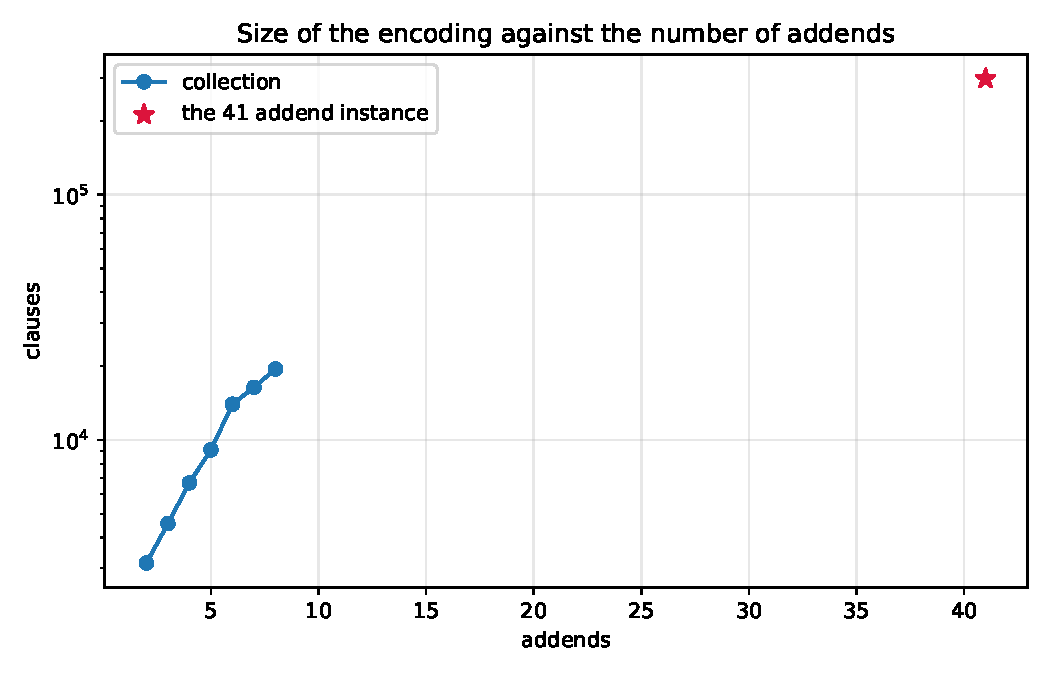
\includegraphics[width=0.72\textwidth]{figures/clauses_vs_addends.pdf}
\caption{Mean size of the encoding against the number of addends, with the
instance from the task page marked.}
\label{fig:clauses}
\end{figure}

Figure~\ref{fig:clauses} extends the same picture to the instance posed by the
task page. The growth is steady across the collection and the marked point
sits far above it, since that instance has 41 addends where the collection
reaches eight.

\subsection*{The instance posed by the task page}

\begin{table}[H]
\centering
\begin{tabular}{lrrrrrrr}
\toprule
asked for & variables & clauses & solutions & calls & encode [s] & solve [s] & total [s] \\
\midrule
first solution & 48\,480 & 297\,651 & 1 & 1 & 0.21 & 3.38 & 3.59 \\
uniqueness & 48\,480 & 297\,651 & 1 & 2 & 0.20 & 4.87 & 5.08 \\
all solutions & 48\,480 & 297\,651 & 1 & 2 & 0.21 & 5.02 & 5.22 \\
\bottomrule
\end{tabular}
\caption{The 41 addend instance under the three options. Each row is the
median of five runs, the spread between the fastest and the slowest search
being under $10\%$ in every mode.}
\label{tab:bench}
\end{table}

Table~\ref{tab:bench} answers the question the task page asks. Finding one
solution takes $3.6$ seconds and proving that it is the only one takes $5.1$,
the difference being the second call which has to show that no other
assignment works. Enumerating all solutions costs the same as deciding
uniqueness here, because there is only one solution to find.

The instance is timed five times per mode because a single measurement of it
is not reliable. Repeated on an otherwise idle machine the search time varies
by only a few per cent, but the same runs taken while the machine was busy
were slower by a factor of two, which is enough to change the answer to the
question the task asks. The counts do not move at all: the encoding is
$48\,480$ variables and $297\,651$ clauses on every run.

The instance has 41 addends, 31 distinct words and 10 distinct letters,
\code{AEHMNORSTY}, so for $k=10$ under the one-to-one requirement the letters
use every digit once. The solution is
\[
  \code{E}=0,\ \code{O}=1,\ \code{M}=2,\ \code{S}=3,\ \code{Y}=4,\
  \code{H}=5,\ \code{N}=6,\ \code{A}=7,\ \code{R}=8,\ \code{T}=9,
\]
giving $\code{TESTS} = 90393$, which was checked against the sum of the 41
decoded addends.

Compared with the collection this instance is two orders of magnitude larger,
$297\,651$ clauses against a mean of $4\,708$, and building the clause list
still takes a fraction of a second while the solver needs several.

\begin{figure}[H]
\centering
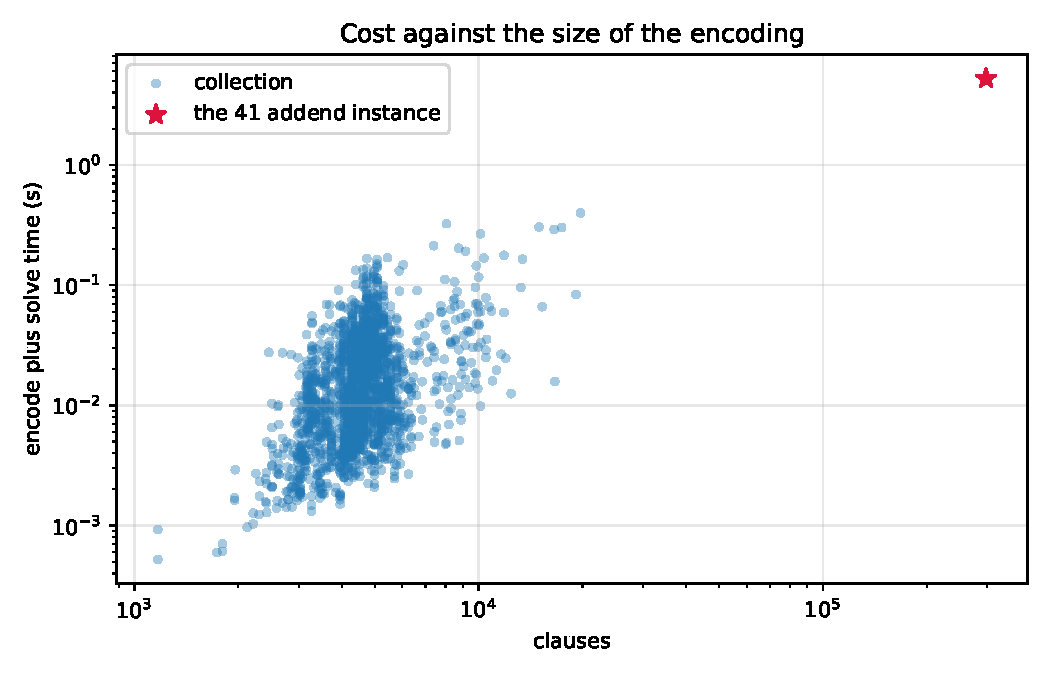
\includegraphics[width=0.72\textwidth]{figures/time_vs_clauses.pdf}
\caption{Cost against the size of the encoding, both axes logarithmic, over
every puzzle of the collection with the instance from the task page marked.}
\label{fig:time}
\end{figure}

Figure~\ref{fig:time} plots every puzzle. The spread at a fixed size is wide,
about an order of magnitude, so the number of clauses predicts the cost only
loosely and the difficulty of the individual puzzle matters as much.

\begin{figure}[H]
\centering
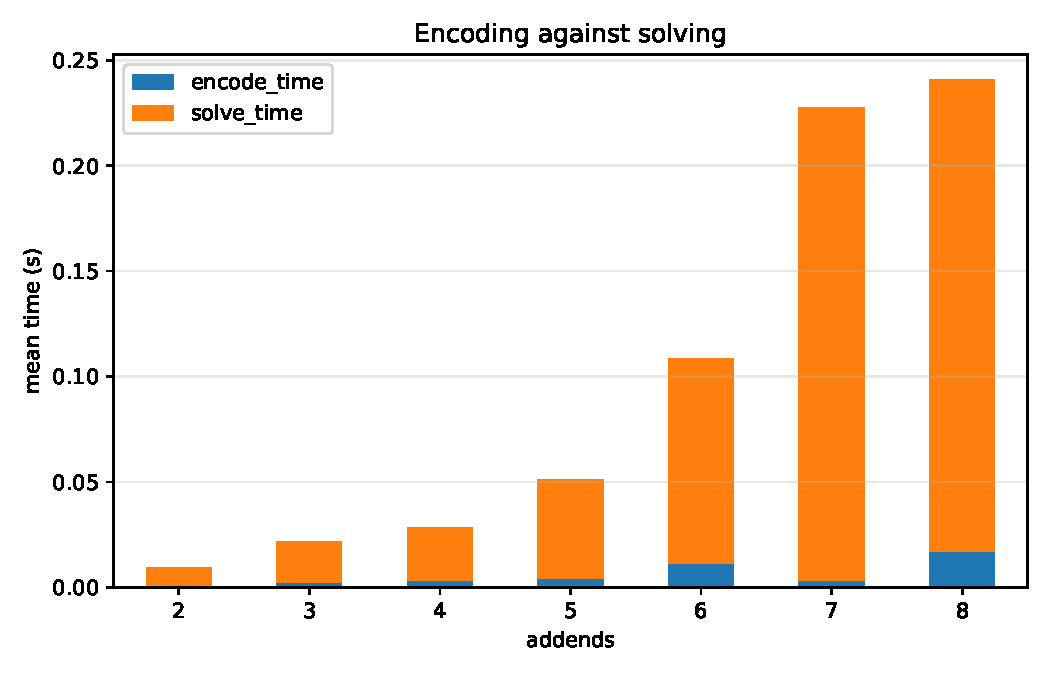
\includegraphics[width=0.72\textwidth]{figures/phases.pdf}
\caption{Encoding against solving, mean over the collection by number of
addends.}
\label{fig:phases}
\end{figure}

Figure~\ref{fig:phases} separates the two phases. Building the clause list in
Python stays a small part of the total at every size, so the measurement
describes the solver rather than the implementation around it.

\subsection*{Options and their cost}

Both options were run over the whole collection and agreed on all $1997$
puzzles. They also cost the same, and the reason is a property of these
instances rather than of the implementation. The collection was generated to
contain puzzles with one solution, so the cut-off at the second model is never
reached: both modes make one call that returns the solution, add the clause
forbidding it, and make a second call that comes back unsatisfiable. The calls
column of \code{results.csv} is $2$ on every one of the $1997$ rows in both
modes, so any difference in wall clock between them is run to run variation
and not a saving.

The cut-off is still worth having, and the place to see it is a formula with
many solutions rather than this collection. Deciding uniqueness costs two
calls whatever the number of solutions, while enumerating them costs one call
per solution plus one. On \code{AB+BA=CD} with repeated digits allowed, which
has $36$ solutions, that is $2$ calls against $37$. The collection cannot show
this, since it deliberately contains no such puzzle.

\subsection*{Code}

All code is in \code{cryptarithms/code/} and is available in the
repository~\cite{repo}.

\begin{itemize}
  \item \code{cryptarithm.py} holds the equation parser, the one-hot integers
  with their addition and carry splitting, the encoder and the enumeration
  loop. It also provides the check for uniqueness, which stops at the second
  solution.

  \item \code{formula.py} holds the boolean structure, the parser for
  \code{AND}, \code{OR} and \code{NOT}, and the encoding that gives every
  equation a variable and joins them.

  \item \code{instances.py} reads the collection files, recovering the
  expected digit of every letter from the solution printed beside each puzzle.

  \item \code{test\_cryptarithm.py} contains the checks: the comparison
  against enumerating every assignment, the other bases, the leading zero
  rule, the connectives, the published assignments and the uniqueness of the
  collection.

  \item \code{bench.py} runs the sweep and records the size of the encoding,
  the number of solutions, the calls and the times.

  \item \code{experiments.ipynb} runs everything and writes \code{results.csv}
  and the figures used here.
\end{itemize}

The command line takes a formula and the options, for example
\code{python cryptarithm.py "SEND+MORE=MONEY" -{}-all} or
\code{python cryptarithm.py "A+B=C OR D+E=F" -{}-base 8 -{}-repeat}.

\subsection*{Summary}

The encoding uses one-hot variables for the letters and for the
column sums and carries, and similar constructions. That choice keeps every constraint the task
asks for cheap to state: a letter takes one digit, two letters differ, a word
does not begin with zero, and a column total splits into a written digit and a
carry, the last of these needing two clauses per value and no arithmetic
circuit. The carry is a one-hot integer like everything else, so the same
encoding handles both a puzzle with two addends and the instance with 41,
where the carry reaches 40.

All the features the task lists are implemented and checked. The base ($k$) is a
parameter, verified against enumeration for values 5, 8, 10, 12 and 16. The
one-to-one reading is optional and is the only constraint the option removes.
Solutions can be counted or enumerated, and uniqueness can be decided in two
calls whatever the number of solutions, though on this collection that saves
nothing because every puzzle in it has one solution. Equations combine with \code{AND}, \code{OR} and
\code{NOT}, which requires each equation to be tied to a variable in both
directions so that it can be negated.

Over the collection of $1997$ puzzles every published assignment was recovered
and every puzzle was confirmed to have one solution, in $45.5$ seconds
altogether. The instance posed by the task page is solved in $3.6$ seconds and
proved unique in $5.1$, each the median of five runs.

The measurements also show what the encoding is sensitive to. The number of
letters is nearly constant across the collection, so it is the number of
addends that drives the size, both because each addend adds a term to every
column and because it widens the range of the partial sums that represent
those columns. That is the cost of representing sums in one-hot rather than in
binary, and it is the first thing that would have to change for instances much
larger than the one asked about.

\clearpage

\begin{thebibliography}{9}

\bibitem{tamura}
N. Tamura, \emph{Cryptarithm puzzles}.
\url{https://tamura70.gitlab.io/web-puzzle/cryptarithm/}

\bibitem{pysat}
A. Ignatiev, A. Morgado, J. Marques-Silva,
\emph{PySAT: A Python Toolkit for Prototyping with SAT Oracles}, SAT 2018.
\url{https://pysathq.github.io}

\bibitem{cadical}
A. Biere, \emph{CaDiCaL}.
\url{http://fmv.jku.at/cadical}

\bibitem{repo}
Z. Ahmetovic, source code for this task.
\url{https://github.com/inferno73/SAT-solver-NAIL094}

\end{thebibliography}

\end{document}
